\section{Throwing Booth}
\label{sec:booth}
The booth is constructed from Item Profiles.
The objects are thrown through in front of a constant background, therefore there is a white back wall opposite the camera.
When creating the booth design, care was taken to ensure that the size corresponds to the width of a table (750mm).
This also defined the distance between the camera and the back wall.
With the opening angle of the lens, the minimum required size of the back wall can be calculated as in equation \ref{eq:Fieldwith}. 
In the following this size is called field of view.

\begin{equation}
	f_\text{w} = 2 \cdot a \cdot \tan\left( \frac{\vartheta}{2}\right) = \SI{690}{mm}
	\label{eq:Fieldwith}
\end{equation}

Whereby the following applies:
\begin{itemize}
	\item $f_\text{w}$ = width of the field of view
	\item $a$ = Distance camera to back panel = \SI{630}{mm}
	\item $\vartheta$ = horizontal angle of view = \SI{57.4}{\degree} \cite{BaumerLense}
\end{itemize}

Assuming that the picture format is 1280 $\times$ \SI{1024}{px}, the height of the field of view ($f_\text{h}$) is equal to

\begin{equation}
	f_\text{h} = f_\text{w} \cdot \frac{\SI{1024}{px}}{\SI{1280}{px}} = \SI{552}{mm}.
	\label{eq:Fieldhight}
\end{equation}

The objects should be passed as far away from the camera as possible to be able to take more pictures per throw.
To ensure that the objects are thrown through the field of view and far away from the camera, there is a hole in the back wall as a target.
It is located on the right side of the back wall, which is further away from the camera.
If the throwing objects are hit through the hole in the rear wall, they land in a net.

The back wall is made of a 5 mm thick plate of ABS.
This material is robust and withstands the impacts of the throwing objects.
The side wall is made of foamed PVC.
Due to the manufacturing process, the plate is less smooth, which results in less light reflections and therefore better pictures.

The whole throwing booth is drawn in the CAD tool Inventor. It is designed with all its components using a 3D model.
The camera is mounted on an Item profile with an aluminum mounting adapter which is shown in figure \ref{fig:mounting_adapter} and protected from damage with an aluminum sheet.
Both components have slotted holes to allow fine adjustments to be made during assembly.
The drawings of these parts can be found in the appendix \ref{app:drawings_camera_protection} and \ref{app:drawings_mounting_adapter}.

\begin{figure}[h]
	\centering
	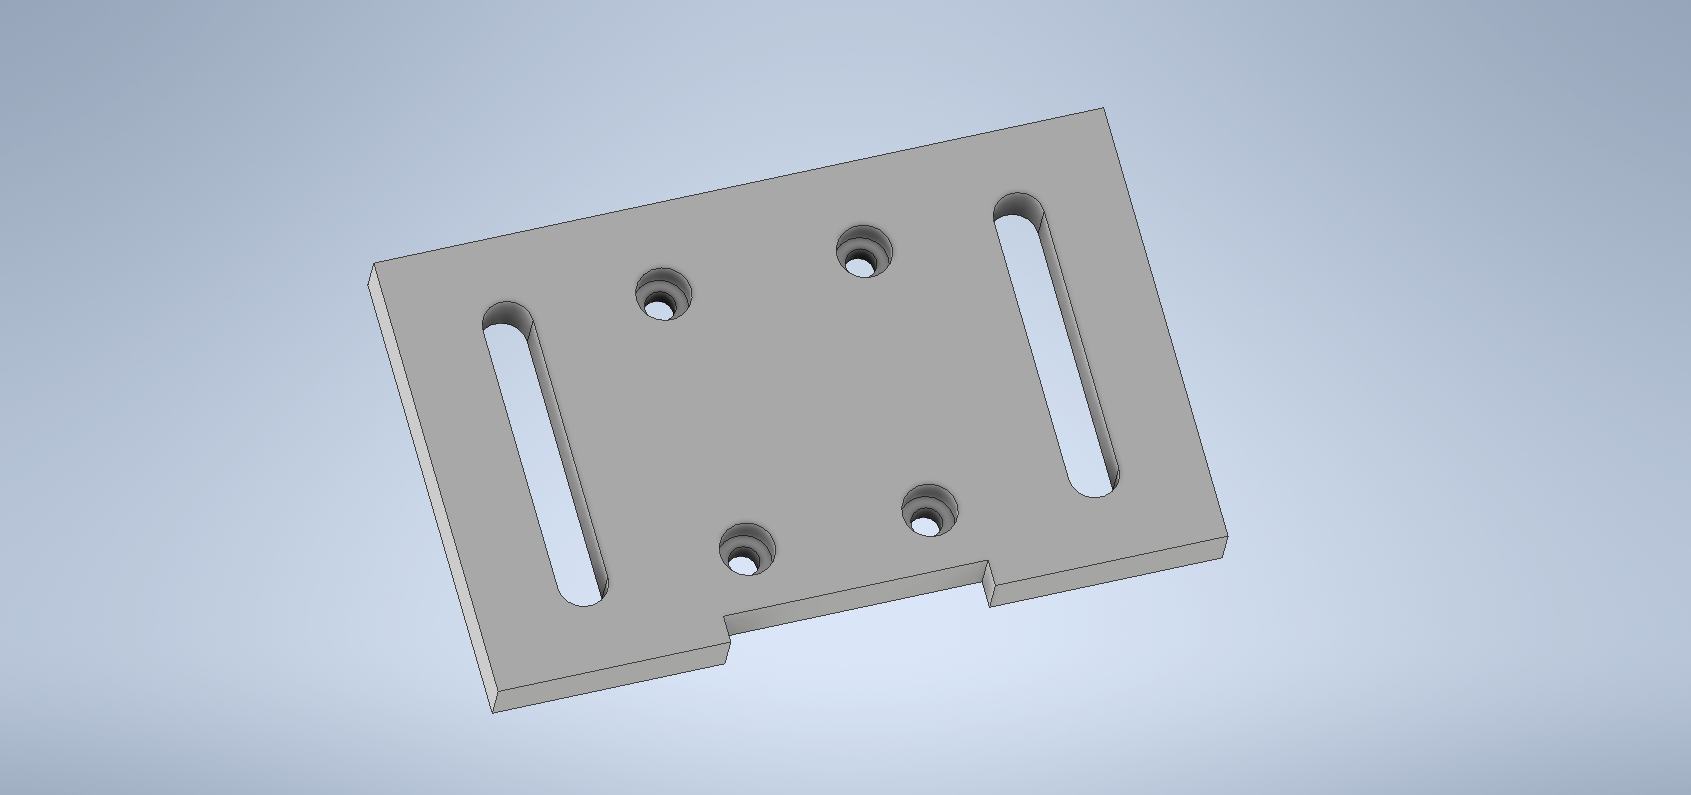
\includegraphics[width=0.4\textwidth]{graphics/mounting_adapter.png}
	\caption{Camera mounting adapter}
	\label{fig:mounting_adapter}
\end{figure}

The power supplies for all electronic components are placed in a box together with the Ultra96-V2.
The box is a case from Fibox with a transparent lid to give visitors an impression of the way it works.
It has a \SI{230}{VAC} power cable, a \SI{24}{VDC} output for lighting, a Mini DisplayPort cable for the monitor, and the USB cable for the camera.
To ensure that the Ultra96-V2 board is cooled, there are also 3 fans on the walls.
The box also contains terminal blocks and cable trunking to store cables that are too long.
Figure \ref{fig:fibox3d} shows the box and the construction drawings for the fibox case can be found in the appendix \ref{app:drawings_fibox_bottom}.

\begin{figure}[h]
	\centering
	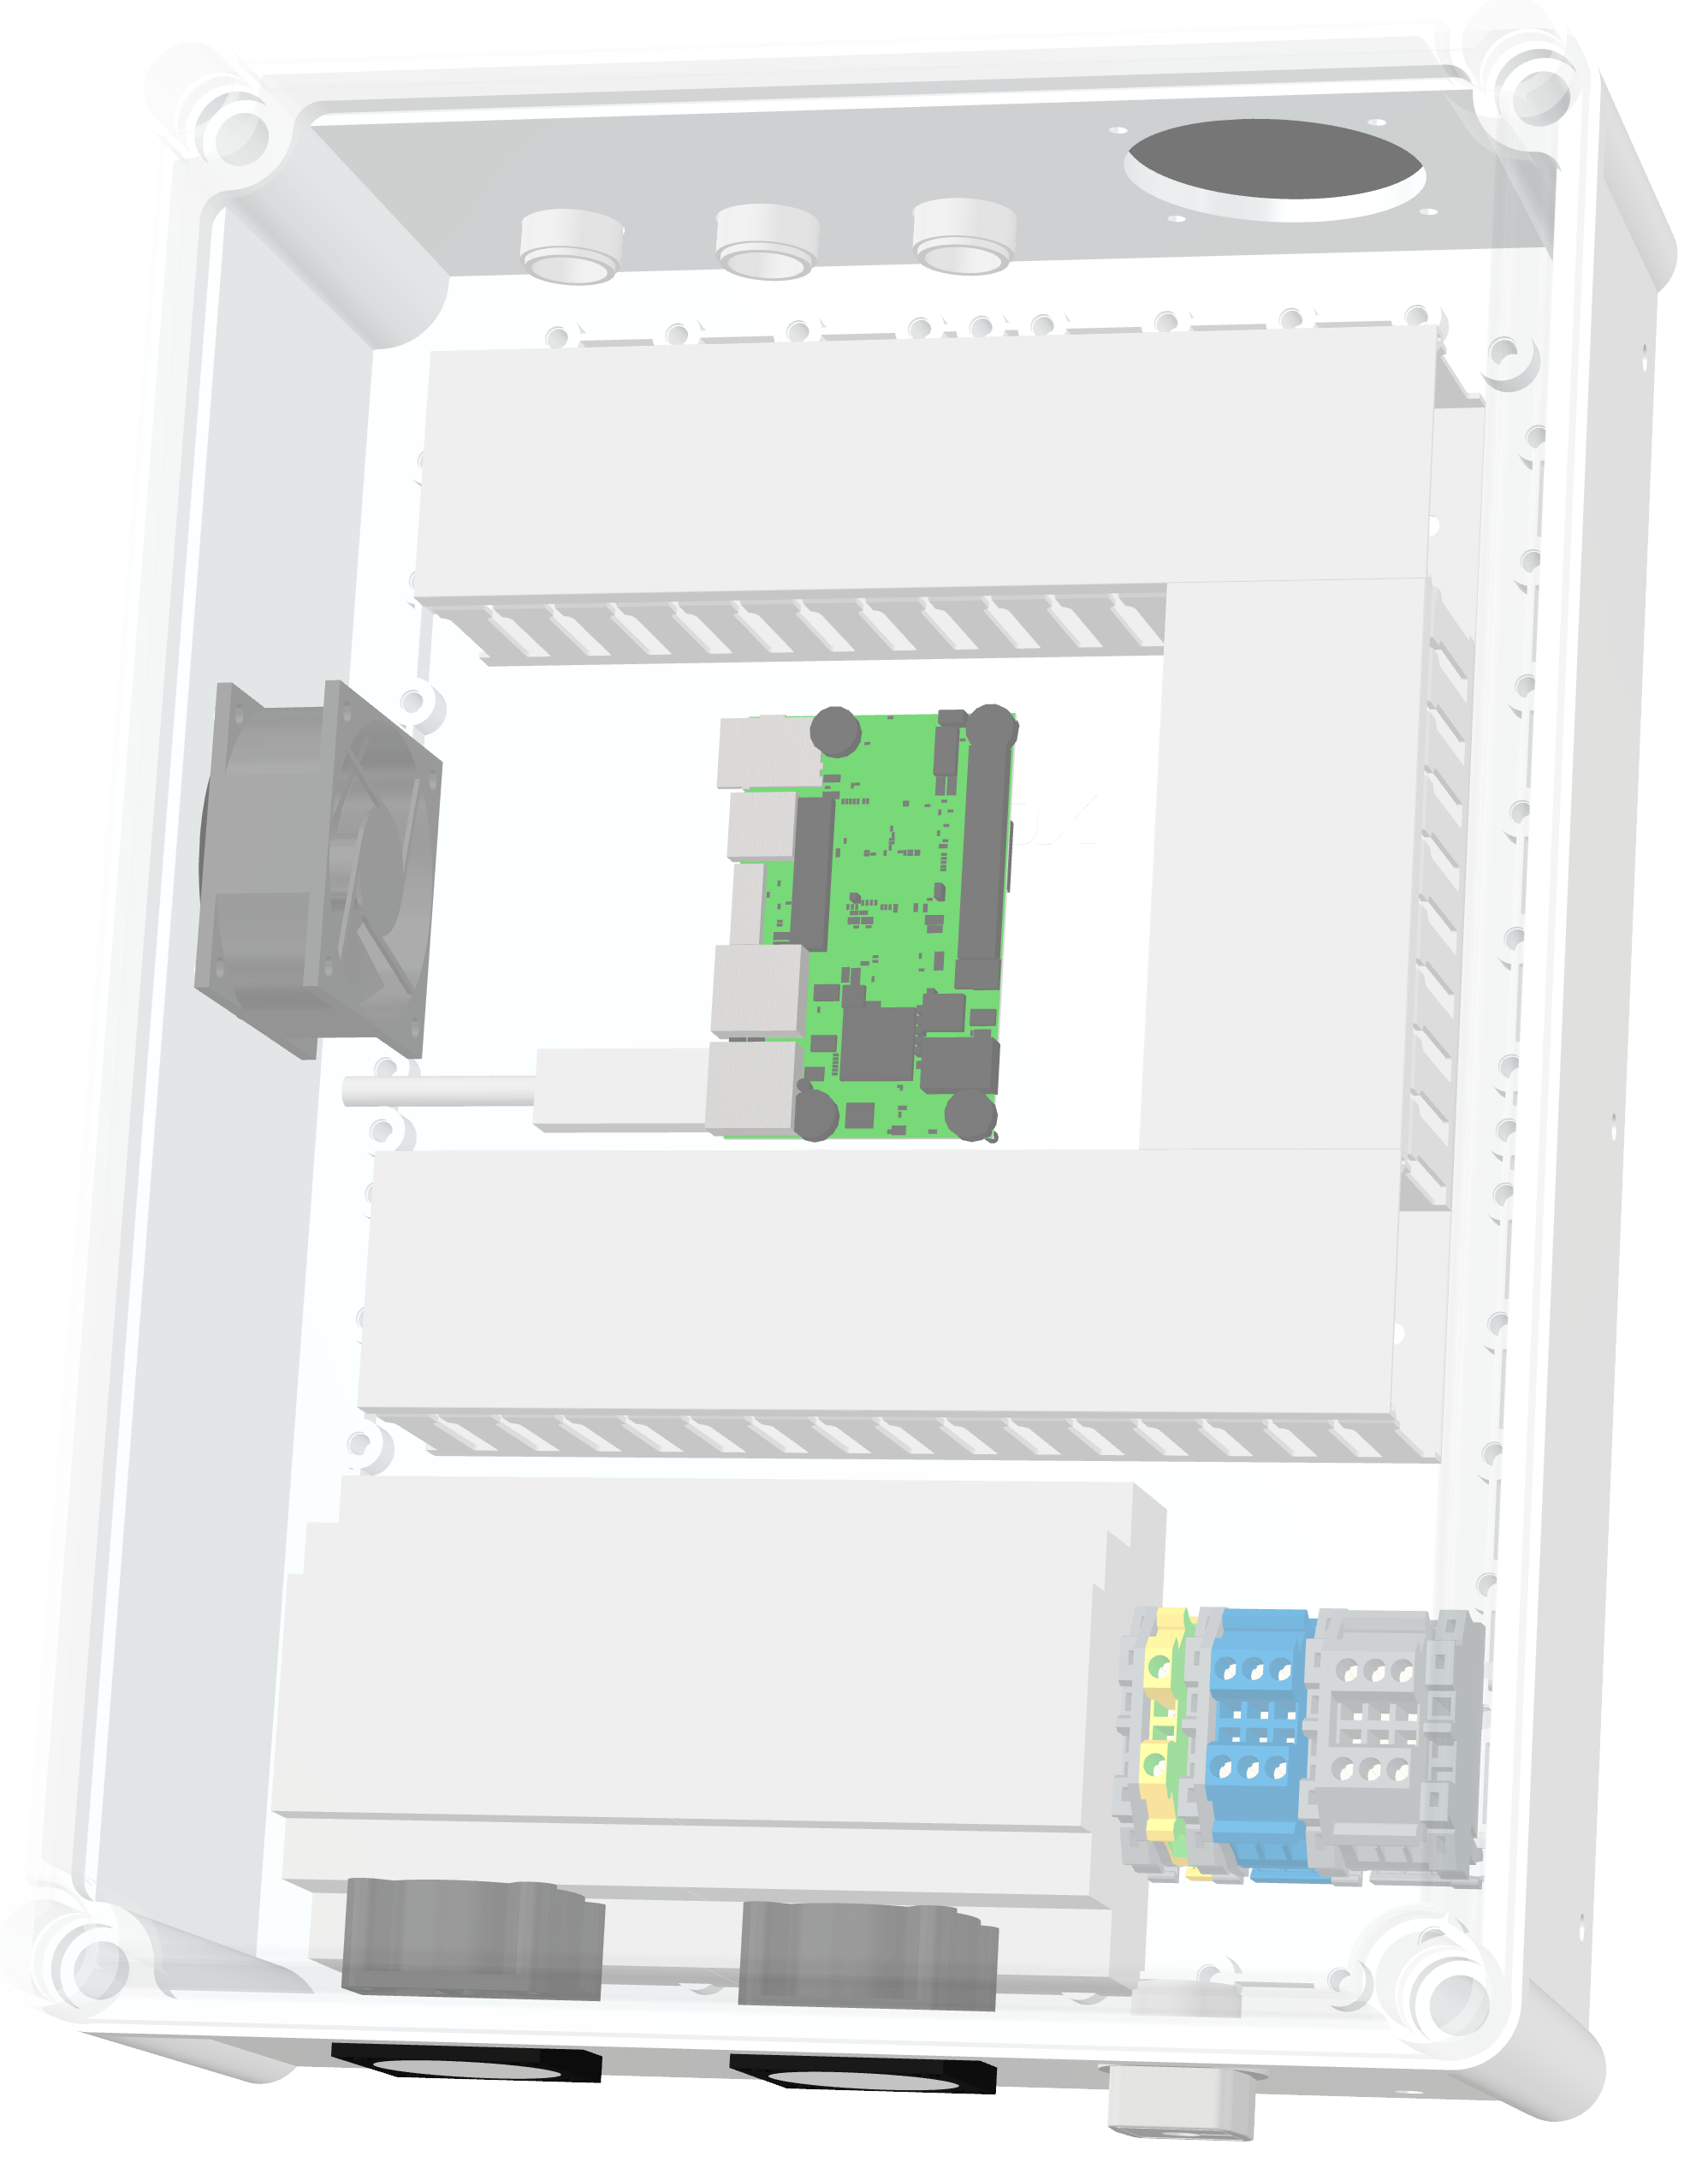
\includegraphics[width=0.3\textwidth]{graphics/case.png}
	\caption{3D Model of the Fibox case}
	\label{fig:fibox3d}
\end{figure}